\documentclass{beamer}
\usepackage[utf8]{inputenc}
\usepackage{multicol}
\usepackage{multirow}
\usepackage{graphics}
\usepackage{tikz}
\usepackage{graphicx}
\usepackage{setspace}
\usepackage{amsthm, amsmath, amsfonts, mathtools, amssymb} % Math packages
\usetheme{Szeged}
\usecolortheme{beaver}
\usefonttheme{structuresmallcapsserif}

\title{The Early History of Game Theory\\
  From Rousseau to Nash}
\author{Mikael Böörs}
\institute{University of Gothenburg}
\date{December 2017}


\begin{document}
 
\frame{\titlepage}

\begin{frame}
\frametitle{Introduction}

What is \emph{Game Theory}?\\~\\

The modern definition of game theory \emph{is
the study of strategic interaction between rational agents}.\\~\\

\begin{itemize}
\item \emph{Strategic interaction}
  \begin{itemize}
    \item The actions of the agents have an impact on the outcome of
      the game for themselves and for the other agents
    \item The agents are aware of this
  \end{itemize}
\item \emph{Rational agents}
    \begin{itemize}
    \item The agents chooses the action that maximizes theirs expected utility
  \end{itemize}
\end{itemize}

 \end{frame}


\begin{frame}
\frametitle{The History of Game Theory}

The mathematical field of game theory is young:

\begin{itemize}
\item Founded by John von Neumann in 1928
  \item Minimax theorem
\end{itemize}

\emph{But} game theoretical problems are old:

\begin{itemize}
\item Philosophers
\item Military strategists
\item Political leaders
\item The common man
\end{itemize}

\end{frame}

\begin{frame}
 
\frametitle{The History of Game Theory}

The mathematical field of game theory is young:

\begin{itemize}
\item Founded by John von Neumann in 1928
  \item Minimax theorem
\end{itemize}

\emph{But} game theoretical problems are old:

\begin{itemize}
\item Philosophers
\item Military strategists
\item Political leaders
\item The common man
\end{itemize}

\end{frame}

\begin{frame}
  
\frametitle{The History of Game Theory}

\emph{Stag Hunt} is a game theoretical problem formulated by Jean-Jacques Rousseau (1712-1778) as a morality problem
of social cooperation.


\begin{table}
  \centering
  \setlength{\extrarowheight}{2pt}
  \scalebox{0.6}{
  \begin{tabular}{cc|c|c|}
    & \multicolumn{1}{c}{} & \multicolumn{2}{c}{Hunter 2}\\
    & \multicolumn{1}{c}{} & \multicolumn{1}{c}{Stag}  & \multicolumn{1}{c}{Hare} \\\cline{3-4}
\multirow{2}*{Hunter 1}  & Stag & (A lot of food, A lot of food) & (No food,A small amount of food) \\\cline{3-4}
    & Hare & (A small amount of food,No food) & (A small amount of food, A small amount of food) \\\cline{3-4}
  \end{tabular}}
\end{table}

\end{frame}

\begin{frame}
  
\frametitle{The History of Game Theory}

\begin{itemize}
\item In 1713 the armature mathematician Francis (?) Waldegrave found the optimal strategy in the card game \emph{le Her}.
  \item In 1913 the German mathematician Ernst Zermelo  published
the first theorem that can be considered a game theoretical
theorem. The theorem that states that in the game of chess, one of the following statements hold:
\begin{itemize}
\item White has a winning strategy
\item Black has a winning strategy
  \item Each of the two players has a strategy guaranteeing at least a
    draw.
  \end{itemize}
\end{itemize}

In 1928 John von Neumann published the article \emph{Zur
      Theorie der Gesellschaftsspiele} where he proved his famous
    \emph{Minimax theorem} that lay the foundation for the modern
    field of game theory. 
\end{frame}

\begin{frame}
  
\frametitle{Strategic Games and the Minimax Theorem}

\begin{table}
  \centering
  \setlength{\extrarowheight}{2pt}
  \scalebox{0.6}{
  \begin{tabular}{cc|c|c|}
    & \multicolumn{1}{c}{} & \multicolumn{2}{c}{Hunter 2}\\
    & \multicolumn{1}{c}{} & \multicolumn{1}{c}{Stag}  & \multicolumn{1}{c}{Hare} \\\cline{3-4}
\multirow{2}*{Hunter 1}  & Stag & (A lot of food, A lot of food) & (No food,A small amount of food) \\\cline{3-4}
    & Hare & (A small amount of food,No food) & (A small amount of food, A small amount of food) \\\cline{3-4}
  \end{tabular}}

  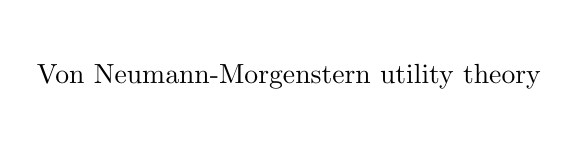
\begin{tikzpicture}
    % nodes
    \node (O) at (0,0) {}; 
    \node (A) at (1, 0) {};
    \node (T) at (1,-0.5) {Von Neumann-Morgenstern utility theory};
\node (B) at (1, -1) {};
    \end{tikzpicture}

  
  \centering
  \setlength{\extrarowheight}{2pt}
    \scalebox{0.6}{
  \begin{tabular}{cc|c|c|}
    & \multicolumn{1}{c}{} & \multicolumn{2}{c}{Player 2}\\
    & \multicolumn{1}{c}{} & \multicolumn{1}{c}{0}  &
                                                              \multicolumn{1}{c}{1}
    \\\cline{3-4}
\multirow{2}*{Player 1}  & 0 & (1, 1) &
                                                                   (-1,0) \\\cline{3-4}
    & 1 & (0, -1) & (0,0) \\\cline{3-4}
  \end{tabular}}
\end{table}

\end{frame}

\begin{frame}
  
  \frametitle{Strategic Games and the Minimax Theorem}

  Zero-sum games

\begin{table}[h!]
  \begin{center}
    \scalebox{0.8}{
    \setlength{\extrarowheight}{2pt}
    \begin{tabular}{cc|c|c|c|}
      & \multicolumn{2}{c}{} & \multicolumn{1}{c}{Player $2$} & \multicolumn{1}{c}{}\\
      & \multicolumn{1}{c}{} & \multicolumn{1}{c}{Rock}  &
                                                          \multicolumn{1}{c}{Paper} & \multicolumn{1}{c}{Scissors} \\\cline{3-5}
      \multirow{2}*{Player $1$}  & Rock & $(0,0)$ & $(-1,1)$ & $(1,-1)$\\\cline{3-5}
      & Paper & $(1,-1)$ & $(0,0)$ & $(-1,1)$\\\cline{3-5}
           \multirow{1}*{}  & Scissors & $(-1,1)$ & $(1,-1)$ & $(0,0)$\\\cline{3-5}   \end{tabular}}
    \end{center}
  \end{table}

Are there any optimal strategies?

\end{frame}

\begin{frame}
  
\frametitle{Strategic Games and the Minimax Theorem}

\begin{theorem}[Minimax]
Let $G = (P,U,S)$ be a strategic zero-sum game with $|P| = 2$ and $|S|
< \infty$ and let $\Gamma (G)$ be the mixed extension of $G$. Then
$\Gamma (G)$ has a value $V$ such that
\begin{equation}
  V = max{\sigma _1 \in
  \Sigma_1} min_{\sigma _2 \in \Sigma_2} \mu_1(\sigma_1,\sigma_2) = min_{\sigma _2 \in
  \Sigma_2} max_{\sigma _1 \in \Sigma_1} \mu_1(\sigma_1,\sigma_2)
\end{equation}
and all mixed strategies $\sigma _1^* \in \Sigma_1$ and $\sigma _2^*
\in \Sigma_2$ such that
\begin{equation}
  \begin{gathered}
\sigma_1^* = argmax_{\sigma _1 \in
  \Sigma_1} min_{\sigma _2 \in \Sigma_2} \mu_1(\sigma_1,\sigma_2)\\
 \sigma_2^* = argmin_{\sigma _2 \in \Sigma_2} max_{\sigma _1 \in
   \Sigma_1} \mu_1(\sigma_1,\sigma_2)
\end{gathered}
\end{equation}
 are optimal mixed strategies for player $1$ and $2$ respectively.
\end{theorem}

\end{frame}

\begin{frame}
  
  \frametitle{Strategic Games and the Minimax Theorem}
\begin{center}
  \includegraphics[width = 7cm]{solving-zero-sum-games-and-the-minimax-theorem__1.jpg}
\end{center}
\end{frame}


\begin{frame}
  
  \frametitle{Equilibria and John Nash}

  
\emph{Prisoners Dilemma}: The game was introduced
by the mathematicians Merrill Flood (1908 – 1991) and Melvin Dresher
(1911-1992) in 1950 who were interested in the applications of game
theory, especially applications regarding nuclear
strategies.

\begin{table}[h!]
  \centering
  \setlength{\extrarowheight}{2pt}
  \begin{tabular}{cc|c|c|}
    & \multicolumn{1}{c}{} & \multicolumn{2}{c}{Player 2}\\
    & \multicolumn{1}{c}{} & \multicolumn{1}{c}{Cooperate}  &
                                                              \multicolumn{1}{c}{Defect}
    \\\cline{3-4}
    \multirow{2}*{Player 1}  & Cooperate & (-1, -1) &
                                                                   (-3,0) \\\cline{3-4}
    & Defect & (0, -3) & (-2,-2) \\\cline{3-4}
  \end{tabular}
\end{table}


\end{frame}


\begin{frame}
  
\frametitle{Equilibria and John Nash}


In 1950 John Forbes Nash (1928-2015) introduced the concept of
  \emph{Nash Equilibria}.

Intuitively, a Nash equilibrium, is a
strategy profile such that none of the player has an incentive to
change strategy. Formally:

\begin{definition}[Nash Equilibrium]
  Given a game $G = (P,U,S)$ with $|S| < \infty$, we say that $s^* \in S$ is a
  \emph{Nash Equilibrium} if $\forall i \in
  \{1,...,|P|\} \text{ and }\forall s_i \in S_i$ $$ u_i(s^*) \geq u_i(s_i,s_{-i}^*).$$ 
\end{definition}


\end{frame}


\begin{frame}
  
\frametitle{Equilibria and John Nash}

\begin{theorem}[Nash's theorem]
  Let $G = (P,U,S)$ be a strategic game with $|P|,|S| < \infty$ and
  let $\Gamma(G)$ be the mixed extension of $G$. $\Gamma(G)$ has at
  least one Nash Equilibrium. 
  \end{theorem}\\~\\

This theorem was published in 1950 and earned Nash the
  Swedish National Bank's Prize in Economic Sciences in Memory of
  Alfred Nobel (not to be confused with a real Nobel Prize!) in 1994.
  
\end{frame}


\begin{frame}
  
  \begin{center}
    \Huge The End
  \end{center}
  
\end{frame}


\end{document}

